\chapter{Implementation of spatial tournaments}
\label{chap:Three}

\section{Introduction}
In this chapter we will discuss the source code committed to the
Axelrod-Python library to implement spatial topology. In addition, some
initial experiments and results will be discussed. These experiments will be
performed using three chosen topologies and two different sizes of competitors.

\subsection{Code Discussion}

As analyzed in \autoref{chap:Two}, the Axelrod library uses a
\texttt{Tournament()} class to run any given tournament. \texttt{Tournament()}
class itself calls upon another class the \texttt{Match Generator()} which is
responsible to generate the matches.
In a round robin case, there is a \texttt{RoundRobinTournament()} class
and a \texttt{RoundRobinMatches()} class that generates matches for each player
against the rest. The parameters and the index of the pair are push to it
by the \texttt{build single match()}. A generator that lives within the class matches.
For a round robin tournament the structure of the code is illustrated in~\ref{fig:rbr}.

\begin{figure}
\centering
    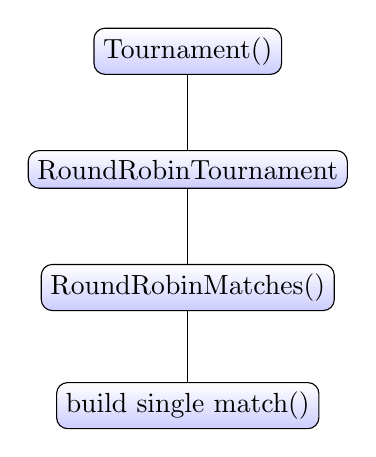
\begin{tikzpicture}[sibling distance=10em,
      every node/.style = {shape=rectangle, rounded corners,
        draw, align=center,
        top color=white, bottom color=blue!20}]]
      \node {Tournament()}
        child { node {RoundRobinTournament}
          child { node {RoundRobinMatches()}
            child { node {build single match()} } }
           };
    \end{tikzpicture}
  \caption{Code structure for a Round Robin tournament.}
  \label{fig:rbr}
\end{figure}

In order for us to implement a Spatial topology tournament we need to follow a
similar approach. Firstly a new \texttt{Match Generator()} class was written.
The \texttt{SpatialMatches()} is a class that generates spatially-structured
matches. In these matches, players interact only with their neighbors rather
than the entire population. According to \cite{Archdeacon1996} graphs can be
represents in many different ways, one of which is by lists of edges.
Due to a various number of python packages that are used for graph manipulation,
we want to keep a more generalized representation of the edges. Thus they will
be passed as a list argument and \texttt{SpatialMatches()} will only create matches
between the ending nodes of these edges. Finally the class \texttt{SpatialTournament()}
runs the spatial tournament. A representation of the code structure now, that
the spatial tournaments have been added, can be seen in Figure~\ref{fig:cds}

\begin{figure}
\centering
    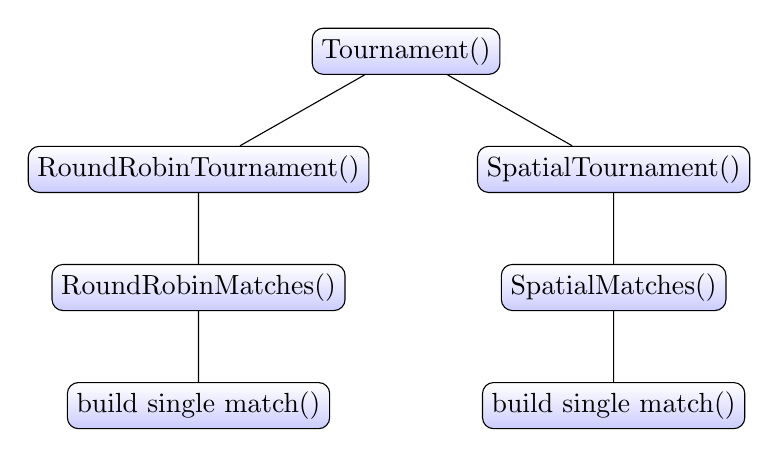
\begin{tikzpicture}[sibling distance=15em,
      every node/.style = {shape=rectangle, rounded corners,
        draw, align=center,
        top color=white, bottom color=blue!20}]]
      \node {Tournament()}
        child { node {RoundRobinTournament()}
          child { node {RoundRobinMatches()}
            child { node {build single match()} } }}
        child { node {SpatialTournament()}
          child { node {SpatialMatches()}
            child { node {build single match()} } }
           };
    \end{tikzpicture}
  \caption{Code structure for when Round Robin and Spatial tournaments are
           implemented.}
  \label{fig:cds}
\end{figure}

In Axelrod library all the components are automatically tested using a
combination of unit, property and integration tests (using \url{travis-ci.org}).
Once a new feature is added to the library, corresponding test must also be written.
The test are used to ensure compatibility and ensure that we get the expected
results. The tests for the \texttt{SpatialTournament()} can be found here :
\url{https://github.com/Axelrod-Python/Axelrod/blob/master/axelrod/tests/unit/test_tournament.py}
under the class \texttt{TestSpatialTournament()}. Anything that was applied to the
library at this point was made possible by using GitHub, a web-based Git repository
hosting service \url{https://github.com/}.


\subsection{Experiment and the three topologies}

In this chapter we will be running some simple examples of spatial topology and
analyze the behavior of the strategies and the results. This will help us further
down to tackle the problem of how topology can affect the outcome of an IPD
competition and which strategies tend to perform well. Some of the most common
networks, based on literature, are a square lattice with four degrees
and a cycle.

In a cycle or circular network consist of a single cycle. It has
equal number of edges and nodes, and each node has degree 2. In~\cite{Szabo2007}
Szabo et all stated that "For spatial models the fixed interaction network is
defined by the sites of a lattice and the edges between those pair whose distance
does not exceed a given value."  The most frequently used structure, and the one
used in this experiment, is the square lattice with von Neumann neighborhood.
Also the most common topology used, again based on literature, is that of a
round robin. A round round topology is nothing else but a complete
graph were every pair of distinct node is connected by a unique edge.
Figure~\ref{fig:networks}, shows an example of all the aforementioned topologies.
Round robin will be mainly used for comparison reasons.

\begin{figure}[h]
\centering
    \begin{subfigure}[t]{0.45\textwidth}
    \centering
        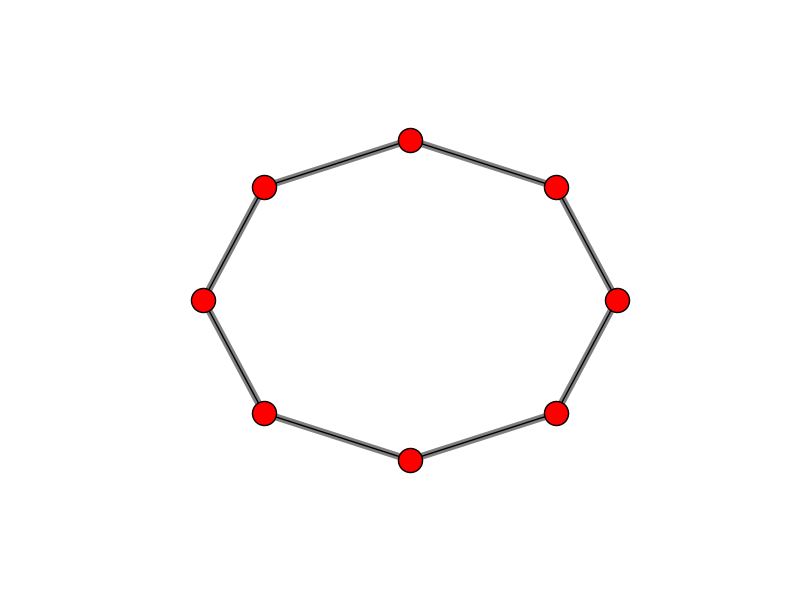
\includegraphics[width=\linewidth]{cycle_network.png}
    \caption{Cycle network.}
    \end{subfigure}
\hfill
    \begin{subfigure}[t]{0.52\textwidth}\centering
    \centering
        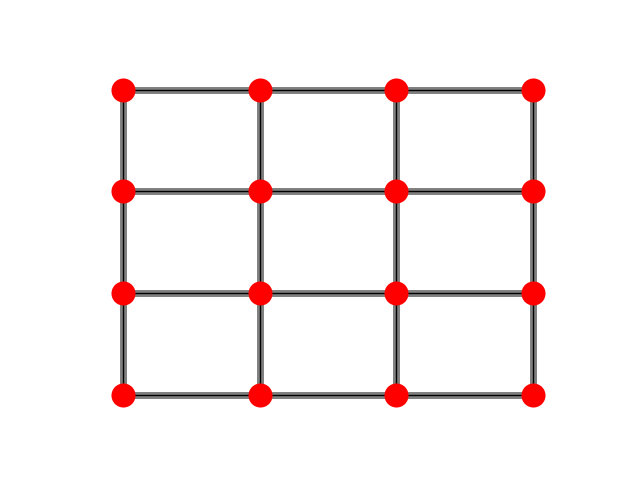
\includegraphics[width=\linewidth]{lattice_network.png}
    \caption{Square lattice with degree 4 network.}
    \end{subfigure}
\hfill
    \begin{subfigure}[t]{0.52\textwidth}\centering
    \centering
        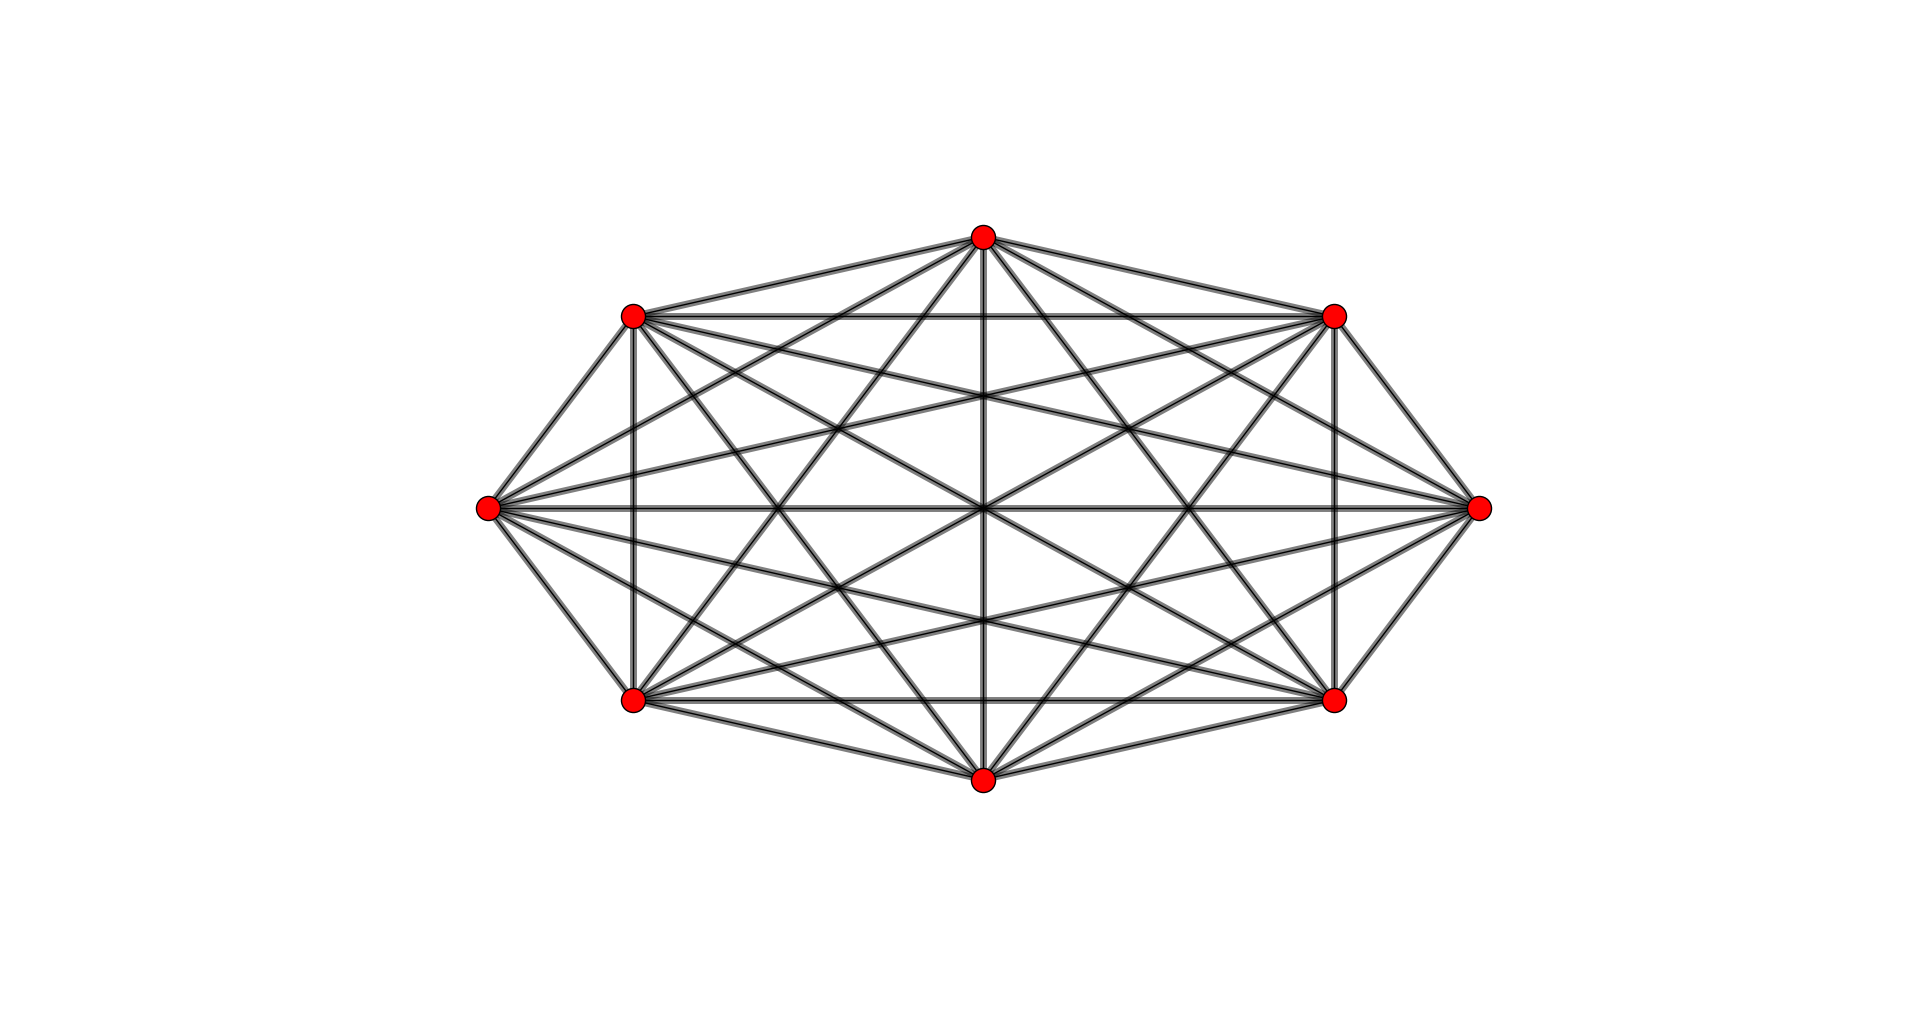
\includegraphics[width=\linewidth]{complete-network.png}
    \caption{A complete or round robin network.}
    \end{subfigure}
\caption{Network topologies.}
\label{fig:networks}
\end{figure}

Thus, we will be performing our experiment with three different topologies, that
of a cycle, a lattice and a complete graph.
For each topology, a fixed size of strategies out of the 132 of Axelrod-Python
library are chosen randomly. These strategies create a neighborhood.
The size of these neighborhoods will range. Let \( s\) be the size of
the neighborhood, where \(s \textrm{ }\{ s=5 \textrm{ and } s=50 \}\).
Subsequently, the strategies are allocated on the graph, based
on the topology, and they compete with their neighbors on a IPD tournament.
For the circular and lattice topology, once the first game is complete,
the strategies are randomly shuffled and allocated on the graph again.
Another tournament is performed this time with different neighbors of a
neighborhood interacting. This is repeated 10 times.
The selection of strategies and creation of neighborhoods is repeated 100 times
and each tournament of an IPD consists of 200 turns and 10 repetitions.

By setting an axelrod-seed~\footnote{A function used by the library, which sets
both seeds for Numpy and the standard library.In general, seeds allow us
reproduce the same players and tournaments.}, the 100 neighborhoods for the
topologies are the same, of course their allocation to the graphs differs because
of the random shuffle.

For the experiments to run we have created three simple scripts, one for every
given topology. This code allow us to generate random
neighborhoods and pass them as nodes on their respective graphs. The tournaments
then are played and produce results. We want to keep track of some given
parameters and to achieve that, the pandas python library is used. We create
a data frame and it allow us to pass all the new values of the parameters that
are produce and afterwards export it to a csv file. Some parameters needed for our
analysis were not given by the Axelrod-Python library, thus a few simple
functions for neighbors and their score were also written.

The Axelrod tournaments themselves make usage of match memory and CPU power and
by adding
these additional rules to the tournaments was only increasing in usage. For that
reason all the tournaments and their results we are run in Raven. Raven is the
master computer of Cardiff University. All the scripts and pbs file, for
communicating with Raven, can be found in my personal GitHub account
\url{https://github.com/Nikoleta-v3}.

% I have to create a repository with all the files for the dissertation and clean
% thing up a little bit. Then I will add the new link here. and a message 'Like my page :D'

\subsection{Initial Analysis}

For each of the experiment we have forced to keep in track for a set of parameters,
such as the list of players in a neighborhood, the score, normalized score and
average score for each strategy etc. From a quick look at these data sets
we can obtain the following informations.

For the spatial tournaments, for both neighborhood sizes (5 and 50)
we achieved 1000 tournaments. Containing 100 different neighborhoods, where each
the exists for 10 tournaments.

Moreover, for the cycle experiment we can see in Table~\ref{sum-cicle}, that degree is
fixed at 2 and the payoffs are fixed to \(R=3, P=1, S=0, T=5\) for both
\( s=5\textrm{ and } s=50 \). For \(s=5\), the mean average score
is 2.45, with a minimum value of 0.0175 and a maximum value of 4.95. The
mean average score of the neighbors score is 980.95 with a standard deviation
of 219.87. Moreover the minimum value is set at 141.55 and the maximum at
1756.50. The mean average score does not seem to differ for \(s=5\),
which is at 2.39. Though, in the experiment with a size of fifty a strategy
achieved a score of 0. Additionally the average score of the neighbors ranges
from 19.30 to 1884.5. In both cases of size the clustering coefficient is zero
and the connectivity due to fixed degree is 2.

\begin{table}[!hbtp]
\centering
\begin{adjustbox}{width=1\textwidth}
\small
\begin{tabular}{@{}|l|l|l|l|l|l|l|l|l|l|@{}}
\toprule
Cycle & \multicolumn{3}{c}{s=5 and s=50}  & \multicolumn{3}{c}{s=5}                              & \multicolumn{3}{c}{s=50}                             \\\midrule
       & (R,P,S,T) & degree & connectivity & average score & average neighbors score & clustering & average score & average neighbors score & clustering \\\midrule
mean   & (3,1,0,5) & 2.0    & 2.0          & 2.456690      & 980.952580              & 0.00       & 2.394577      & 957.238664              & 0.00       \\\midrule
std    & (0,0,0,0) & 0.0    & 0.0          & 0.748772      & 219.875803              & 0.00       & 0.777189      & 231.321350              & 0.00       \\\midrule
min    & (3,1,0,5) & 2.0    & 2.0          & 0.017500      & 141.550000              & 0.00       & 0.000000      & 19.300000               & 0.00       \\\midrule
max    & (3,1,0,5) & 2.0    & 2.0          & 4.950000      & 1756.500000             & 0.00       & 5.000000      & 1884.500000             & 0.00       \\ \bottomrule
\end{tabular}
\end{adjustbox}
\caption{Summary table for topology circle.}
\label{sum-cicle}
\end{table}

For the lattice experiment a table that summarize the data set is shown in Table
~\ref{sum-lattice}. For both size's values the payoffs are the same (\(R=3, P=1, S=0, T=5\))
and the degree is fixed at 4. For \(s=50\) the mean average score
varies between 0.018 and 4.97. The average score of the neighbors varies from
832.67 and 2895.42. Much higher than both the cycle experiments achieve. Logical
based on the fact that the number of neighbors is now doubled. For \(s=5\)
the mean score is 0.57 and the mean average neighbor score 2.45.
The clustering coefficient is 1 and for \(s=50\) is 0.5.
This shows that in the lattice example the strategies tend to create groups.

\begin{table}[!hbtp]
\centering
\begin{adjustbox}{width=1\textwidth}
\small
\begin{tabular}{@{}|l|l|l|l|l|l|l|l|l|l|@{}}
\toprule
Lattice & \multicolumn{3}{c|}{s=5 and s=50} & \multicolumn{3}{c|}{s=5}                             & \multicolumn{3}{c|}{s=50}                            \\ \midrule
       & (R,P,S,T) & degree & connectivity & average score & average neighbors score & clustering & average score & average neighbors score & clustering \\ \midrule
mean   & (3,1,0,5) & 4.0    & 4.0          & 2.450782      & 1958.569220             & 1.0        & 2.393000      & 1912.748200             & 0.5        \\ \midrule
std    & (0,0,0,0) & 0.0    & 0.0          & 0.576812      & 287.638191              & 0.0        & 0.590971      & 268.375436              & 0.00       \\ \midrule
min    & (3,1,0,5) & 4.0    & 4.0          & 0.527500      & 1059.775000             & 1.0        & 0.018750      & 832.675000              & 0.5        \\ \midrule
max    & (3,1,0,5) & 4.0    & 4.0          & 4.245000      & 2518.700000             & 1.0        & 4.973750      & 2895.425000             & 0.5        \\ \bottomrule
\end{tabular}
\end{adjustbox}
\caption{Summary table for topology lattice.}
\label{sum-lattice}
\end{table}

\newpage

Finally, for the round robin tournaments 100 tournaments were performed for both
neighborhood sizes. Parameters such as neighborhood size and neighbor's score
were not computed for the round robin topology. Because all players
interact with each other we would not get any additional information. In
Table~\ref{sum-rr}, we can see the average score the strategies achieved
in this topology for both sizes. In a neighborhood of a size 50, the mean average
score is 2.39 with an standard deviation of 0.335. For \(s=5\) we can notice that the values
are almost equal to those of the lattice topology with \(s=5\).

\begin{table}[H]
\centering
\begin{tabular}{|l|l|l|}
\hline
Round Robin & \multicolumn{1}{c|}{s=5} & \multicolumn{1}{c|}{s=50} \\ \hline
            & average score            & average score             \\ \hline
mean        & 2.447105                 & 2.393220                  \\ \hline
std         & 0.576014                 & 0.335552                  \\ \hline
min         & 0.527500                 & 1.523673                  \\ \hline
max         & 4.245000                 & 3.339592                  \\ \hline
\end{tabular}
\caption{Summary table for round robin topology.}
\label{sum-rr}
\end{table}

In this section we gone through the structure of the source code for implementing
the Spatial Tournament, by adding to the Axelrod-Python library. Furthermore, now
that the code is usable various experiments were conducted with different topologies
and number of players participating in each tournament. An overview of the
data sets produced was done but now in the following sections we will go though
some more analysis on the results.

\newpage
\section{Analyzing the effect of the topologies}
\label{sub:effects}

For all experiments all 132 strategies of Axelrod-Python library have participated
at least in a one tournament. Here we will go through the strategies and their
performance in each experiment. Not all strategies participated in an equal number
of tournaments. Forcing the strategies to perform in a uniform number is not an
option as we want to keep the random effect for validation of the results.
On could argue that by participating in a larger number of tournaments, the
probability of winning increases as well. Thus, instead of number of winning
tournaments our analysis will be using the ratio of wins. By wining ratio we mean
the number of tournaments a strategy got first place divided by the number of tournaments
the strategy competed in. Additionally, the normalized average score each strategy
achieved will also be studied. Mainly to study the variation, helping us to make
conclusions on the perfomance of a strategy.
Lastly, having all different factors such as degree, neighbors, clustering, scores
etc building a regression model could point out effects on the results.

\subsection{Winning Ratio}
\label{sub:winning-ratio}

The winning rations for all three topologies for a neighborhood size equal to
5 are shown in Figure~\ref{fig:winning-five}. In the experiment where the
strategies compete on a cycle topology 124 strategies out of the 132 have a
winning ration greater than zero. The strategies which did not are ALLCorALLD,
Tricky Cooperator, ThueMorseInverse, Hard Tit For 2 Tats,	SolutionB5, Cycler DDC,
Prober and BackStabber. In the lattice topology as well, 8 strategies do not have
a non- zero winning ratio. Fortress4, Bully, Tricky Cooperator, Hard Go
By Majority: 40, 5 and 10. Also Cycler DDC and ALLCorALLD have a similar
performance in this topology as well.
In the round robin tournament various strategies
ranked last, among them Fortress4 and the whole family of Hard Go By Majority.

On the other hand the strategies with the highest winning ration for each
topology are as follow :
\begin{itemize}
  \item Cycle topology with a winning ratio of 0.56 ZD-GEN-2, followed by Punisher
        with 0.55
  \item Lattice topology with a ratio of 0.45 BackStabber and Meta Majority
        Memory one
  \item Round Robin topology with a winning ratio of 1 : Raider, Gradual, Limited
        Retaliate(0.05/20) and BackStabber.
\end{itemize}

In every topology the highest rank strategy between the size five experiments
are different. Only BackStabber seems to be repeated, even so in the third topology
that of a cycle it had a winning ratio of zero. ALLCorALLD, did badly in all
three topologies and the fact that exactly 8 strategies achieved zero
winning ration in lattice and cycle is it not explainable. Though it could be a
coincidence.

Same approach for a neighborhood size of 50. In these experiments
non strategies have a zero ratio. Figure~\ref{fig:winning-fifty}, illustrates the ratios
for each topology in ascending order. The strategies with the highest winning ratio
for each respective topologies are as follow :

\begin{itemize}
  \item Cycle topology with a winning ratio of 1.3 Raider
  \item Lattice topology with a winning ratio of 1.3 Raider
  \item Round Robin topology with a winning ration of 0.833 EvolvedLookerUp
\end{itemize}

Unexpectedly, strategy Raider seems to have first place in both
the cycle and the lattice topology. It achieved a winning ration of 1.3, 0.5
more than the strategy ranked second. Another surprise in the results is
that of the round robin topology. Where almost all strategies have a winning ratio
of zero. Only 14 strategy managed a ratio higher than hero. The strategy with
the highest on of all was EvolvedLookerUp.

Overall, in all six experiments the only strategy that seems to be repeated is
Raider. Compared to all the other strategies that outperformed the rest the seem
to be no similarity in their way of structure and play. Here we could use
a characterization to compare the strategies more efficient. The winning ration
seems to vary from zero to 1.3 and in the round robin topology many strategies
seem to get zero.

% add plot

\begin{figure}[H]
\centering
    \begin{subfigure}[t]{1\textwidth}
    \centering
        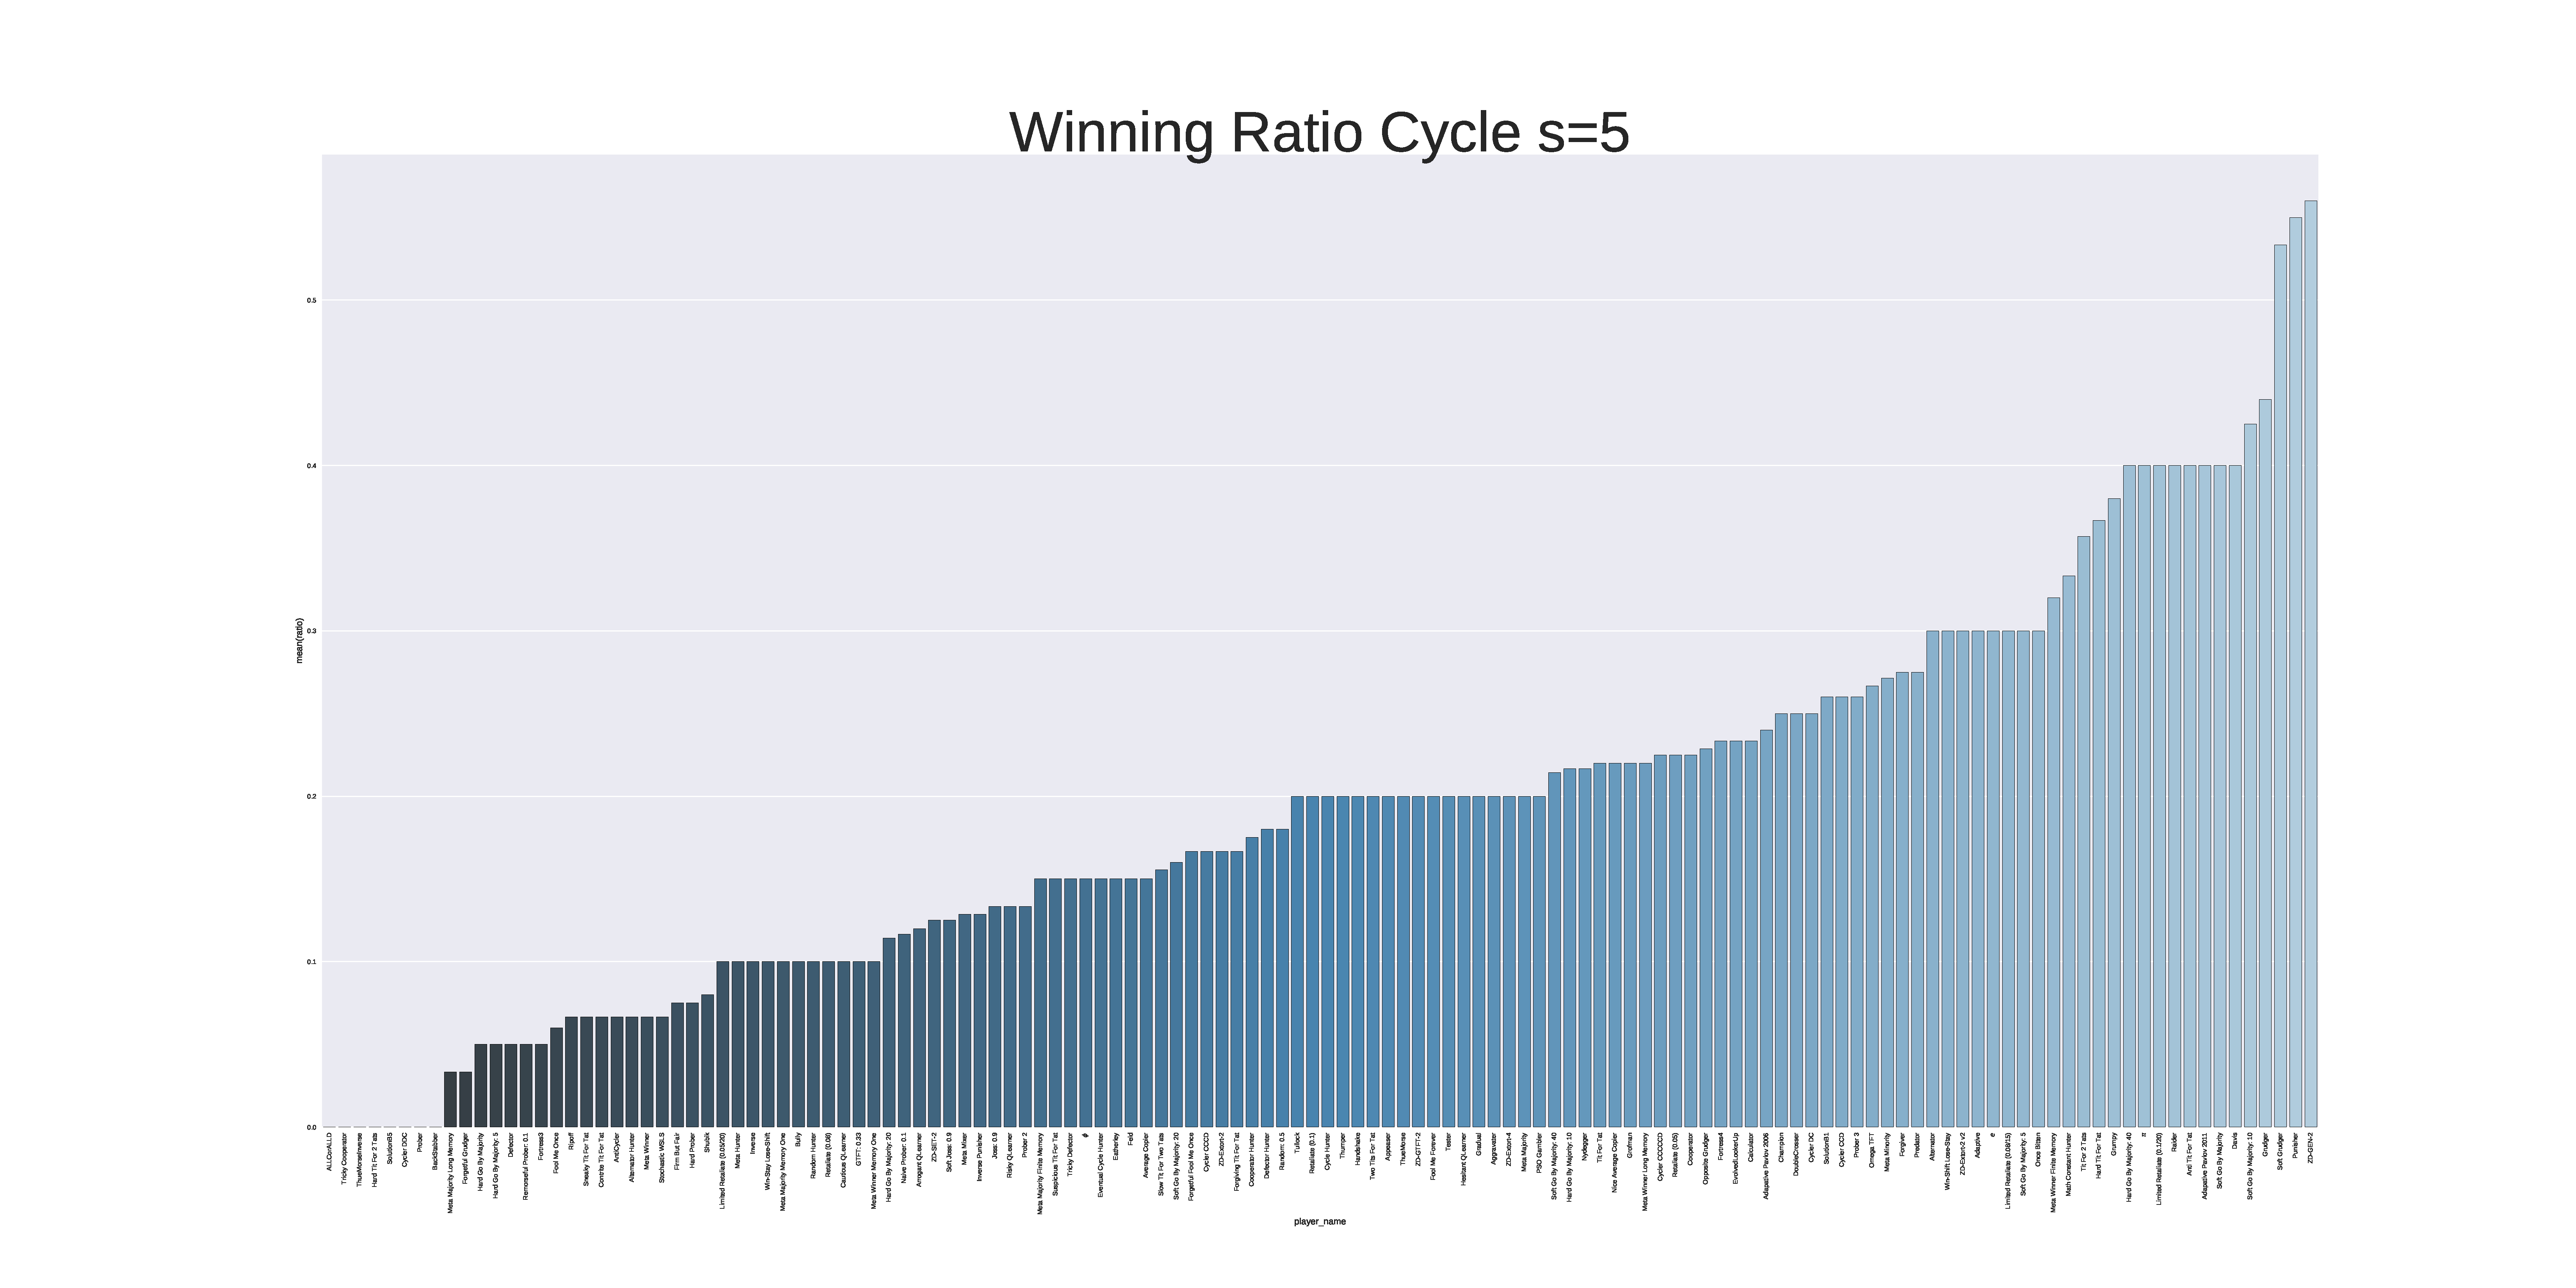
\includegraphics[width=\linewidth]{winners-cycle_five.pdf}
    \caption{Winning ration cycle s=5.}
    \end{subfigure}
\hfill
    \begin{subfigure}[t]{1\textwidth}\centering
    \centering
        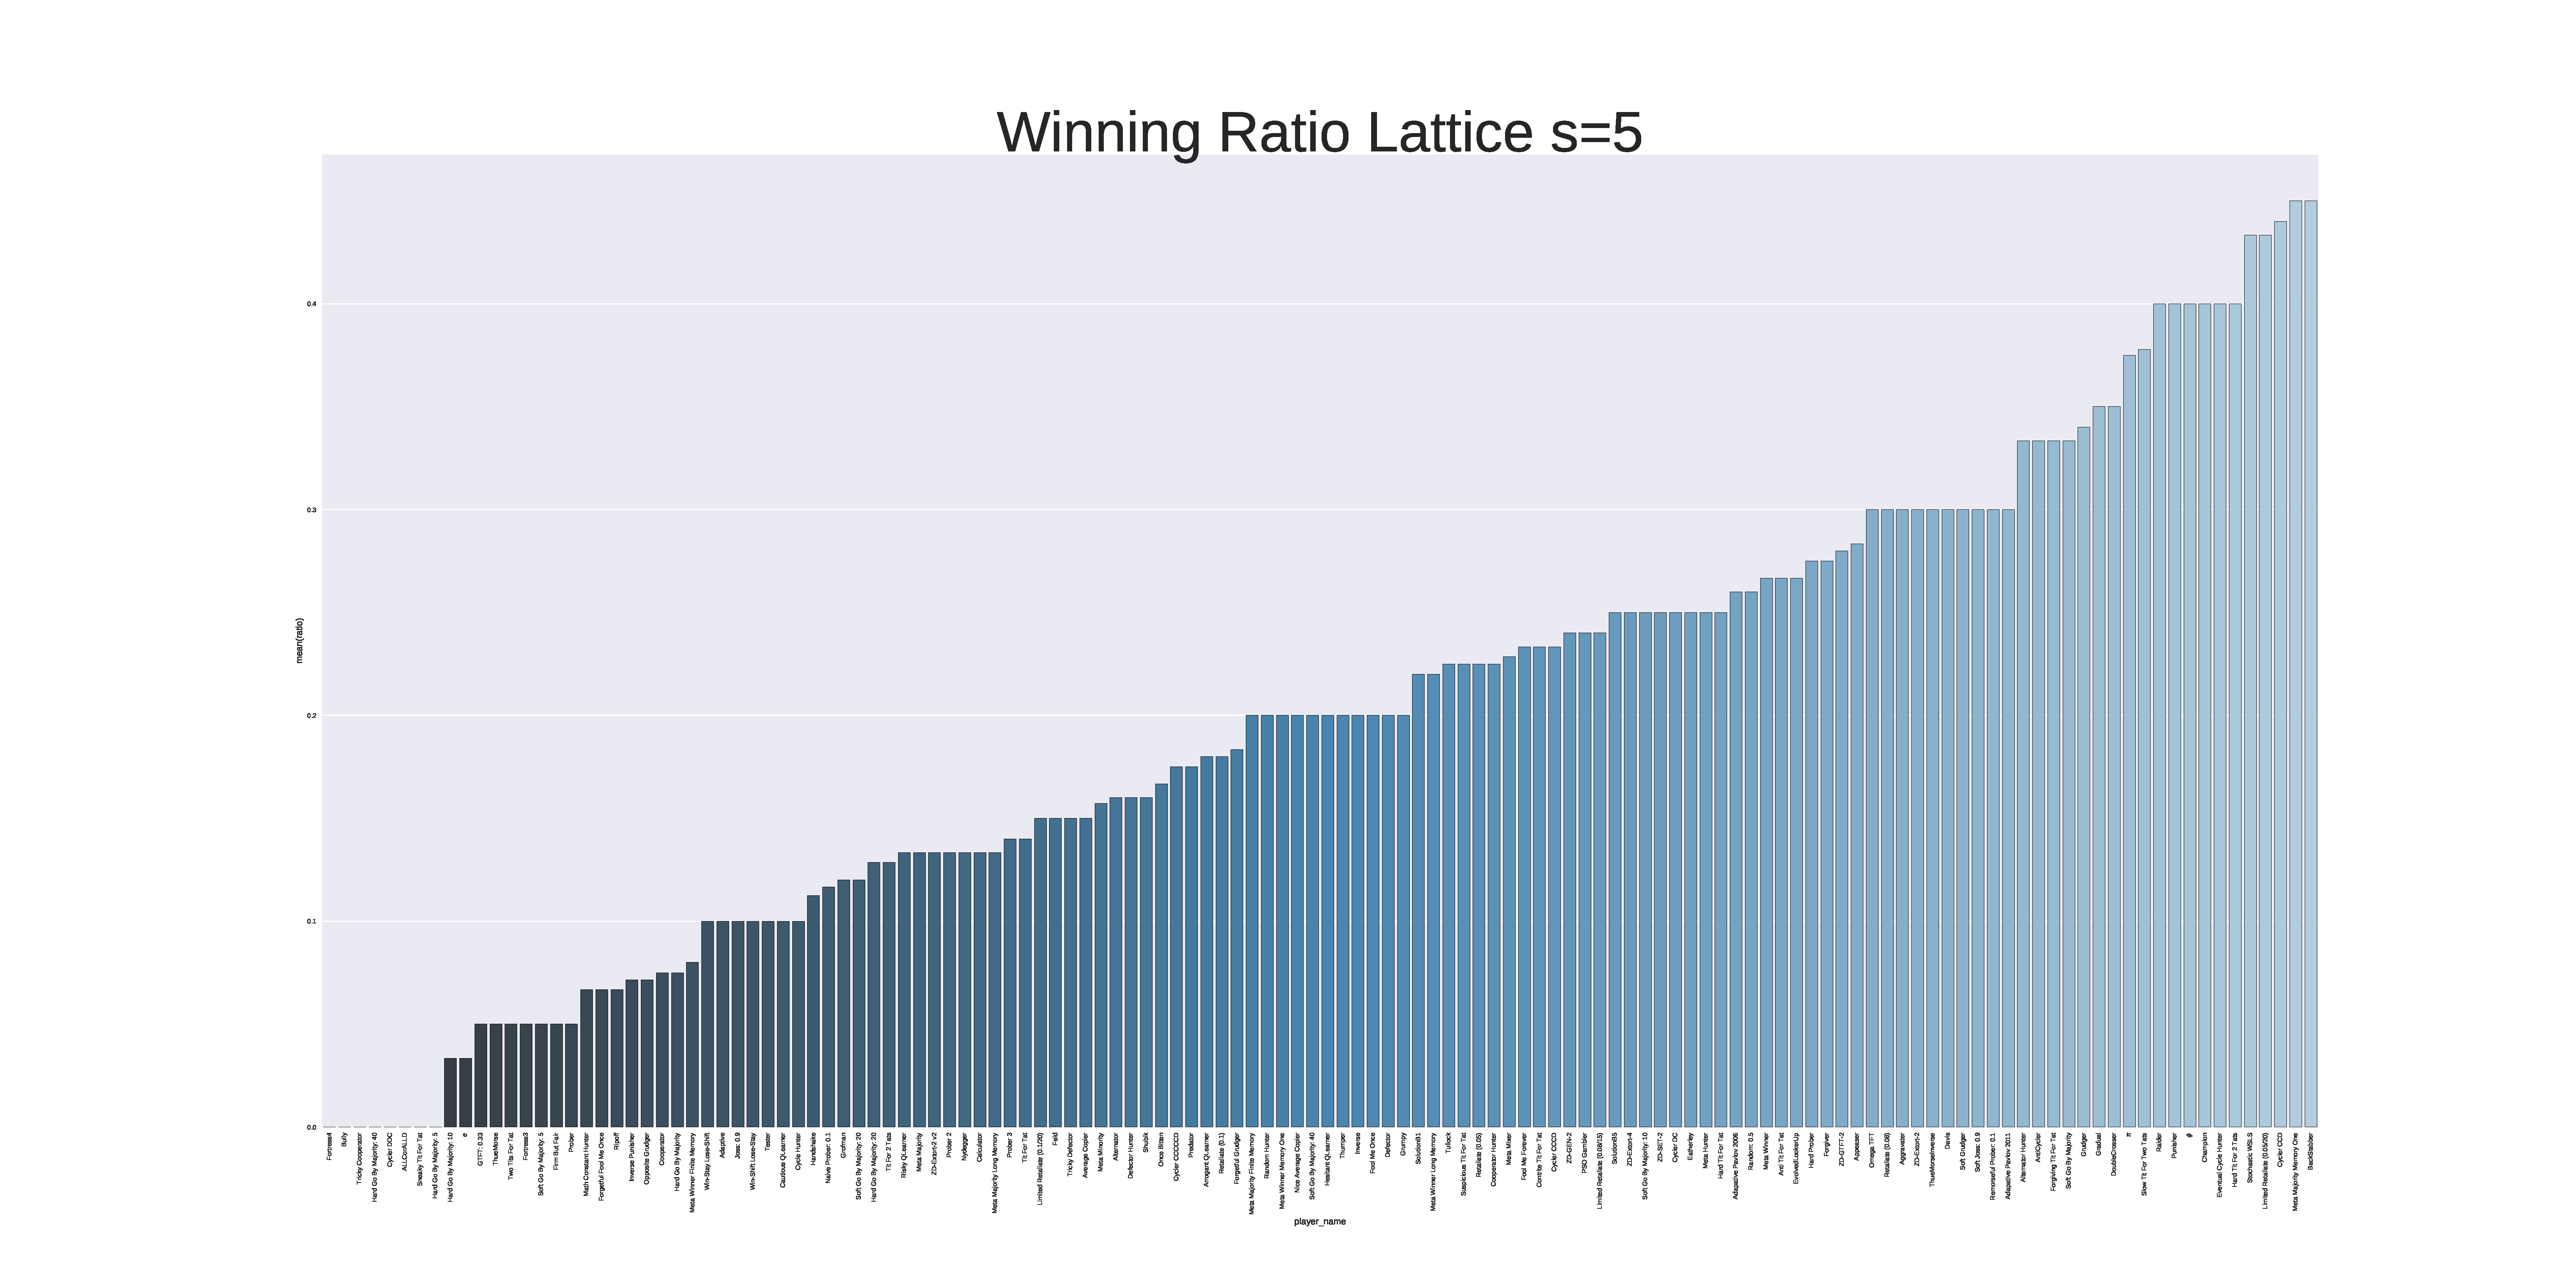
\includegraphics[width=\linewidth]{winners-lattice_five.pdf}
    \caption{Winning ration lattice s=5.}
    \end{subfigure}
\hfill
    \begin{subfigure}[t]{1\textwidth}\centering
    \centering
        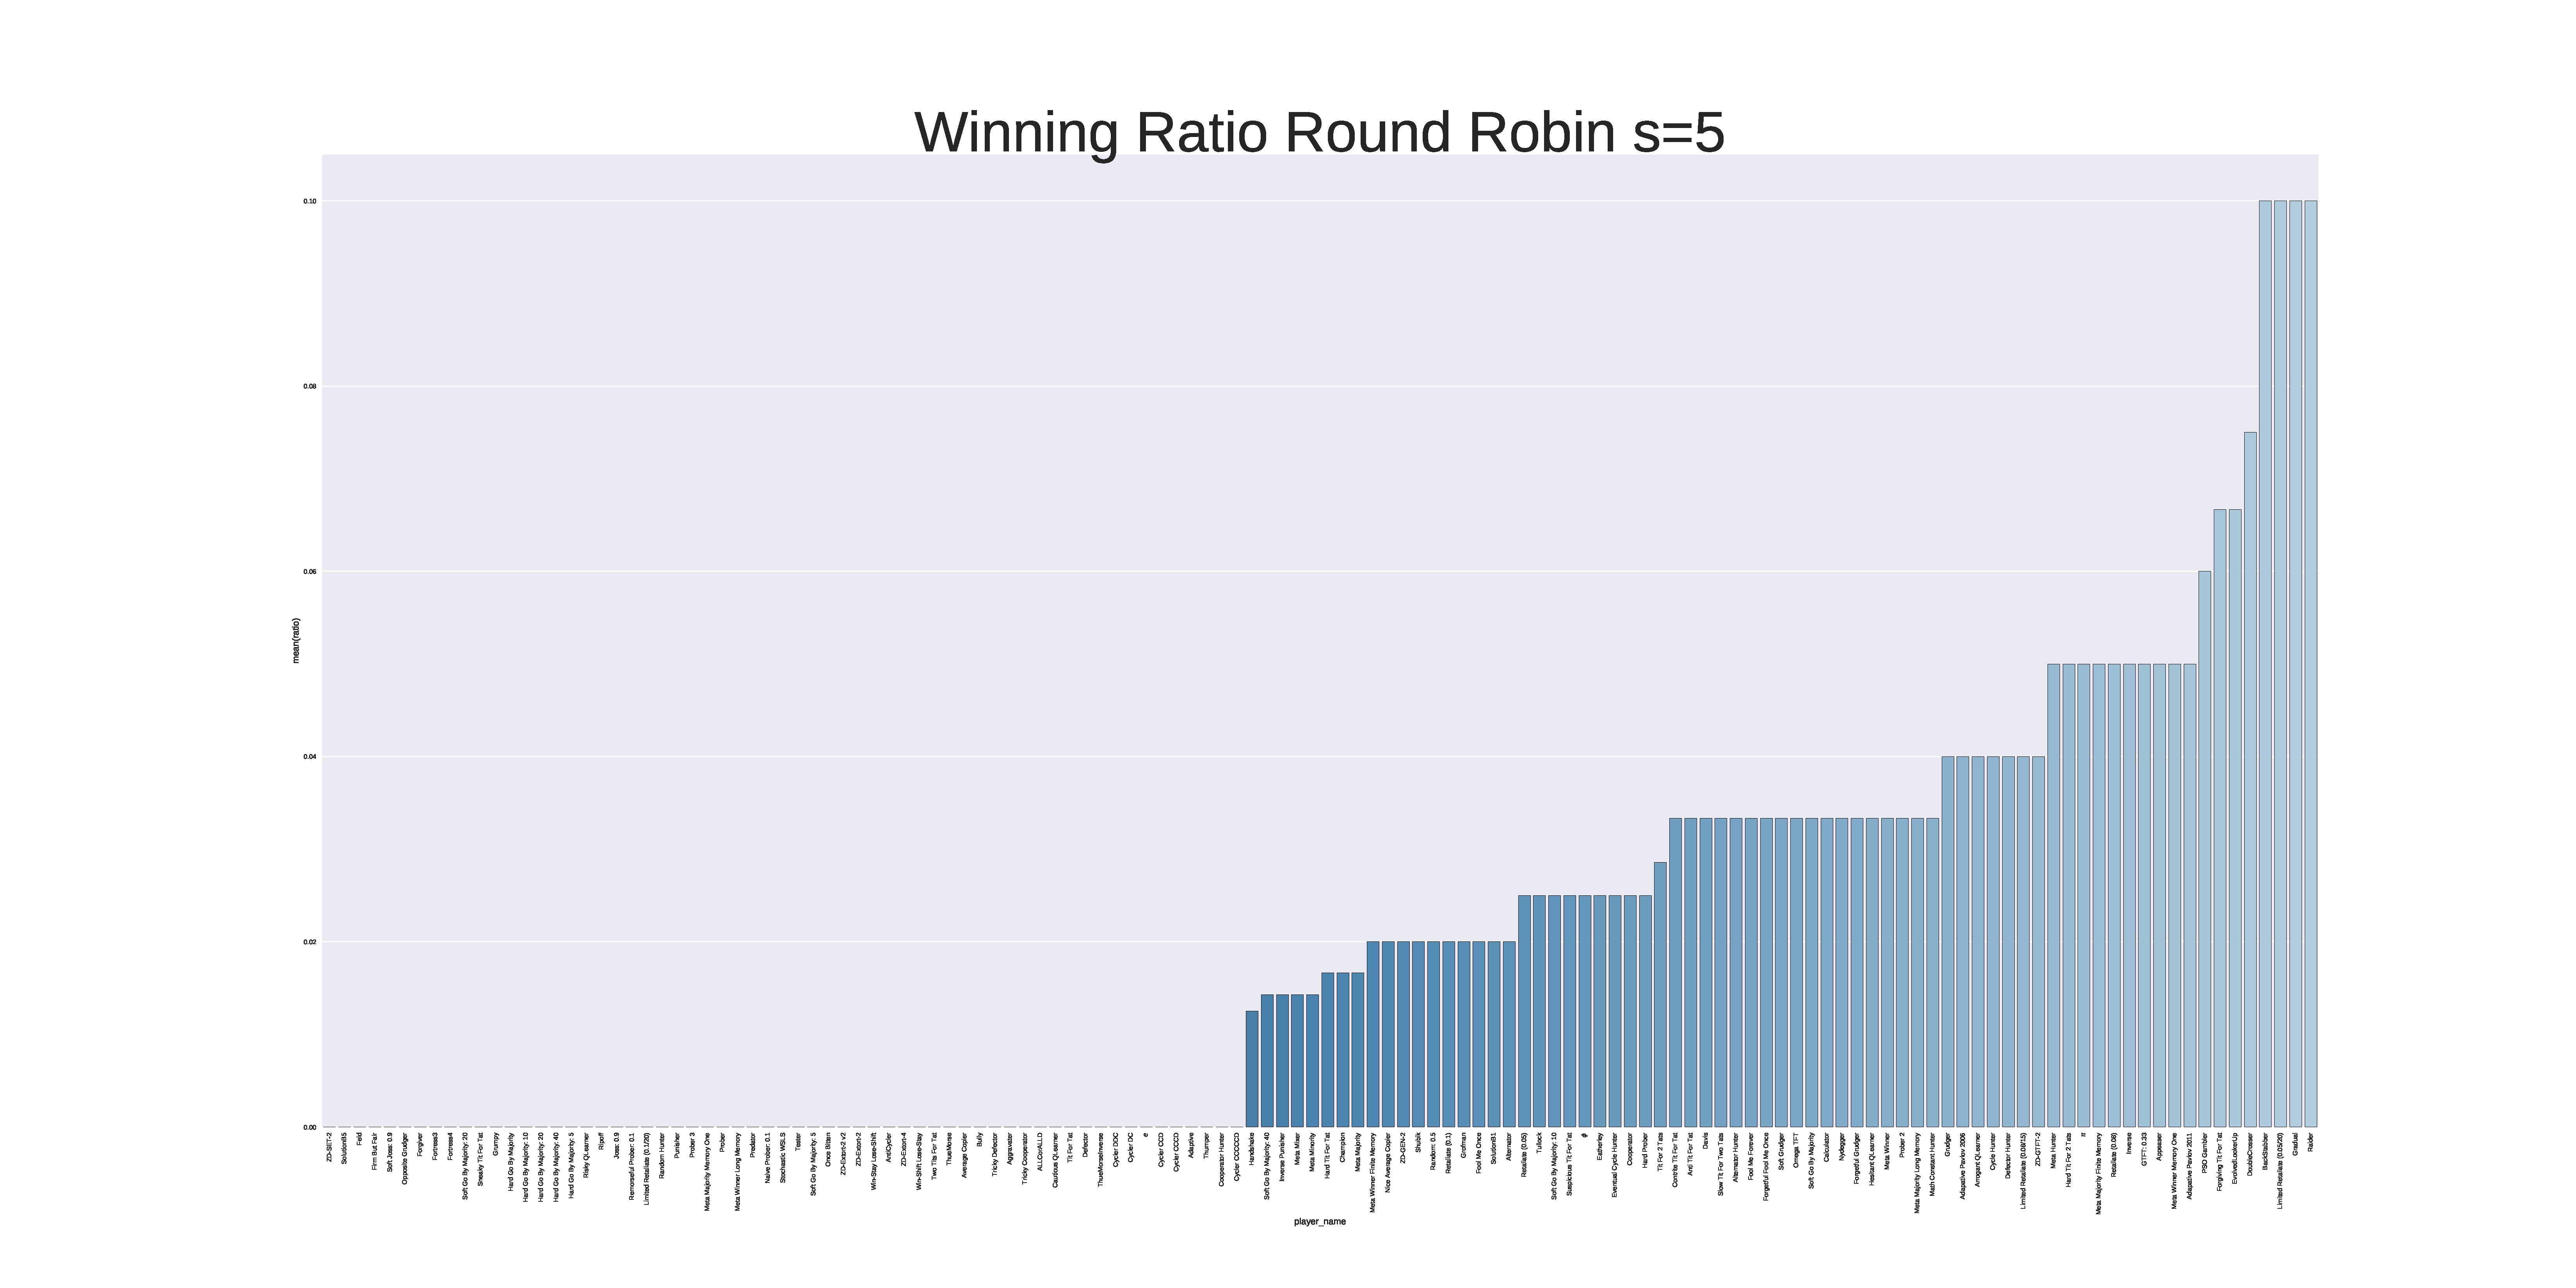
\includegraphics[width=\linewidth]{winners-rr_five.pdf}
    \caption{Winning ration round robin s=5.}
    \end{subfigure}
\caption{Winning ratio for all three topologies s=5.}
\label{fig:winning-five}
\end{figure}

\begin{figure}[H]
\centering
    \begin{subfigure}[t]{1\textwidth}
    \centering
        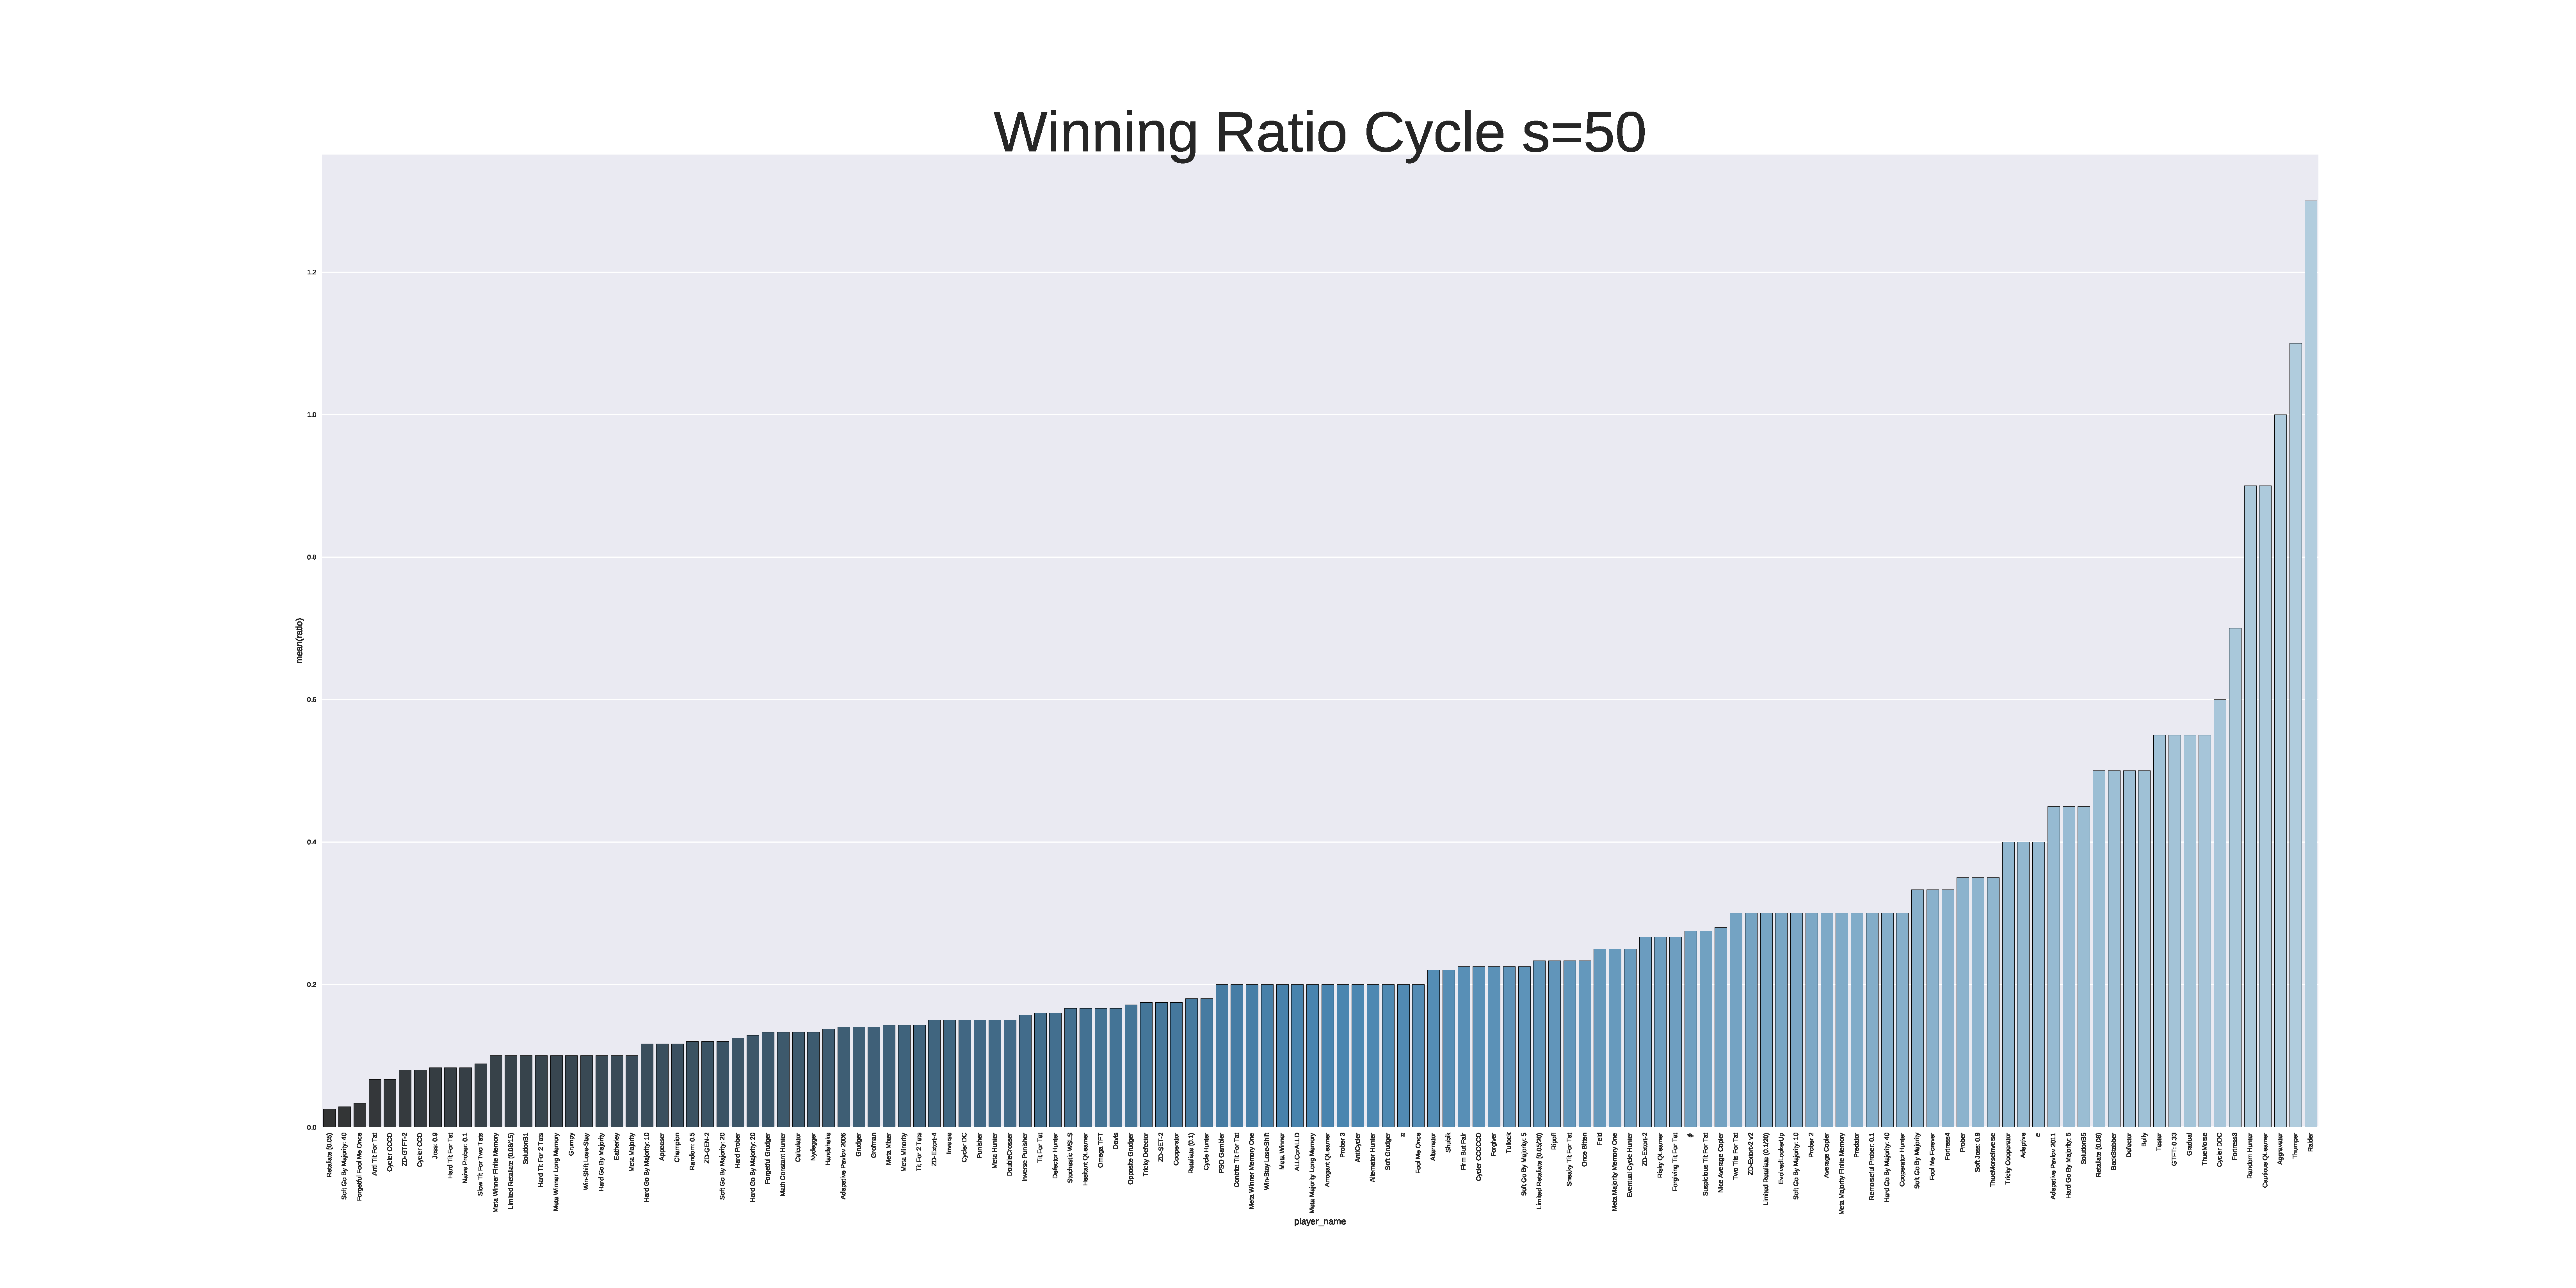
\includegraphics[width=\linewidth]{winners-cycle_fifty.pdf}
    \caption{Winning ration cycle s=50.}
    \end{subfigure}
\hfill
    \begin{subfigure}[t]{1\textwidth}\centering
    \centering
        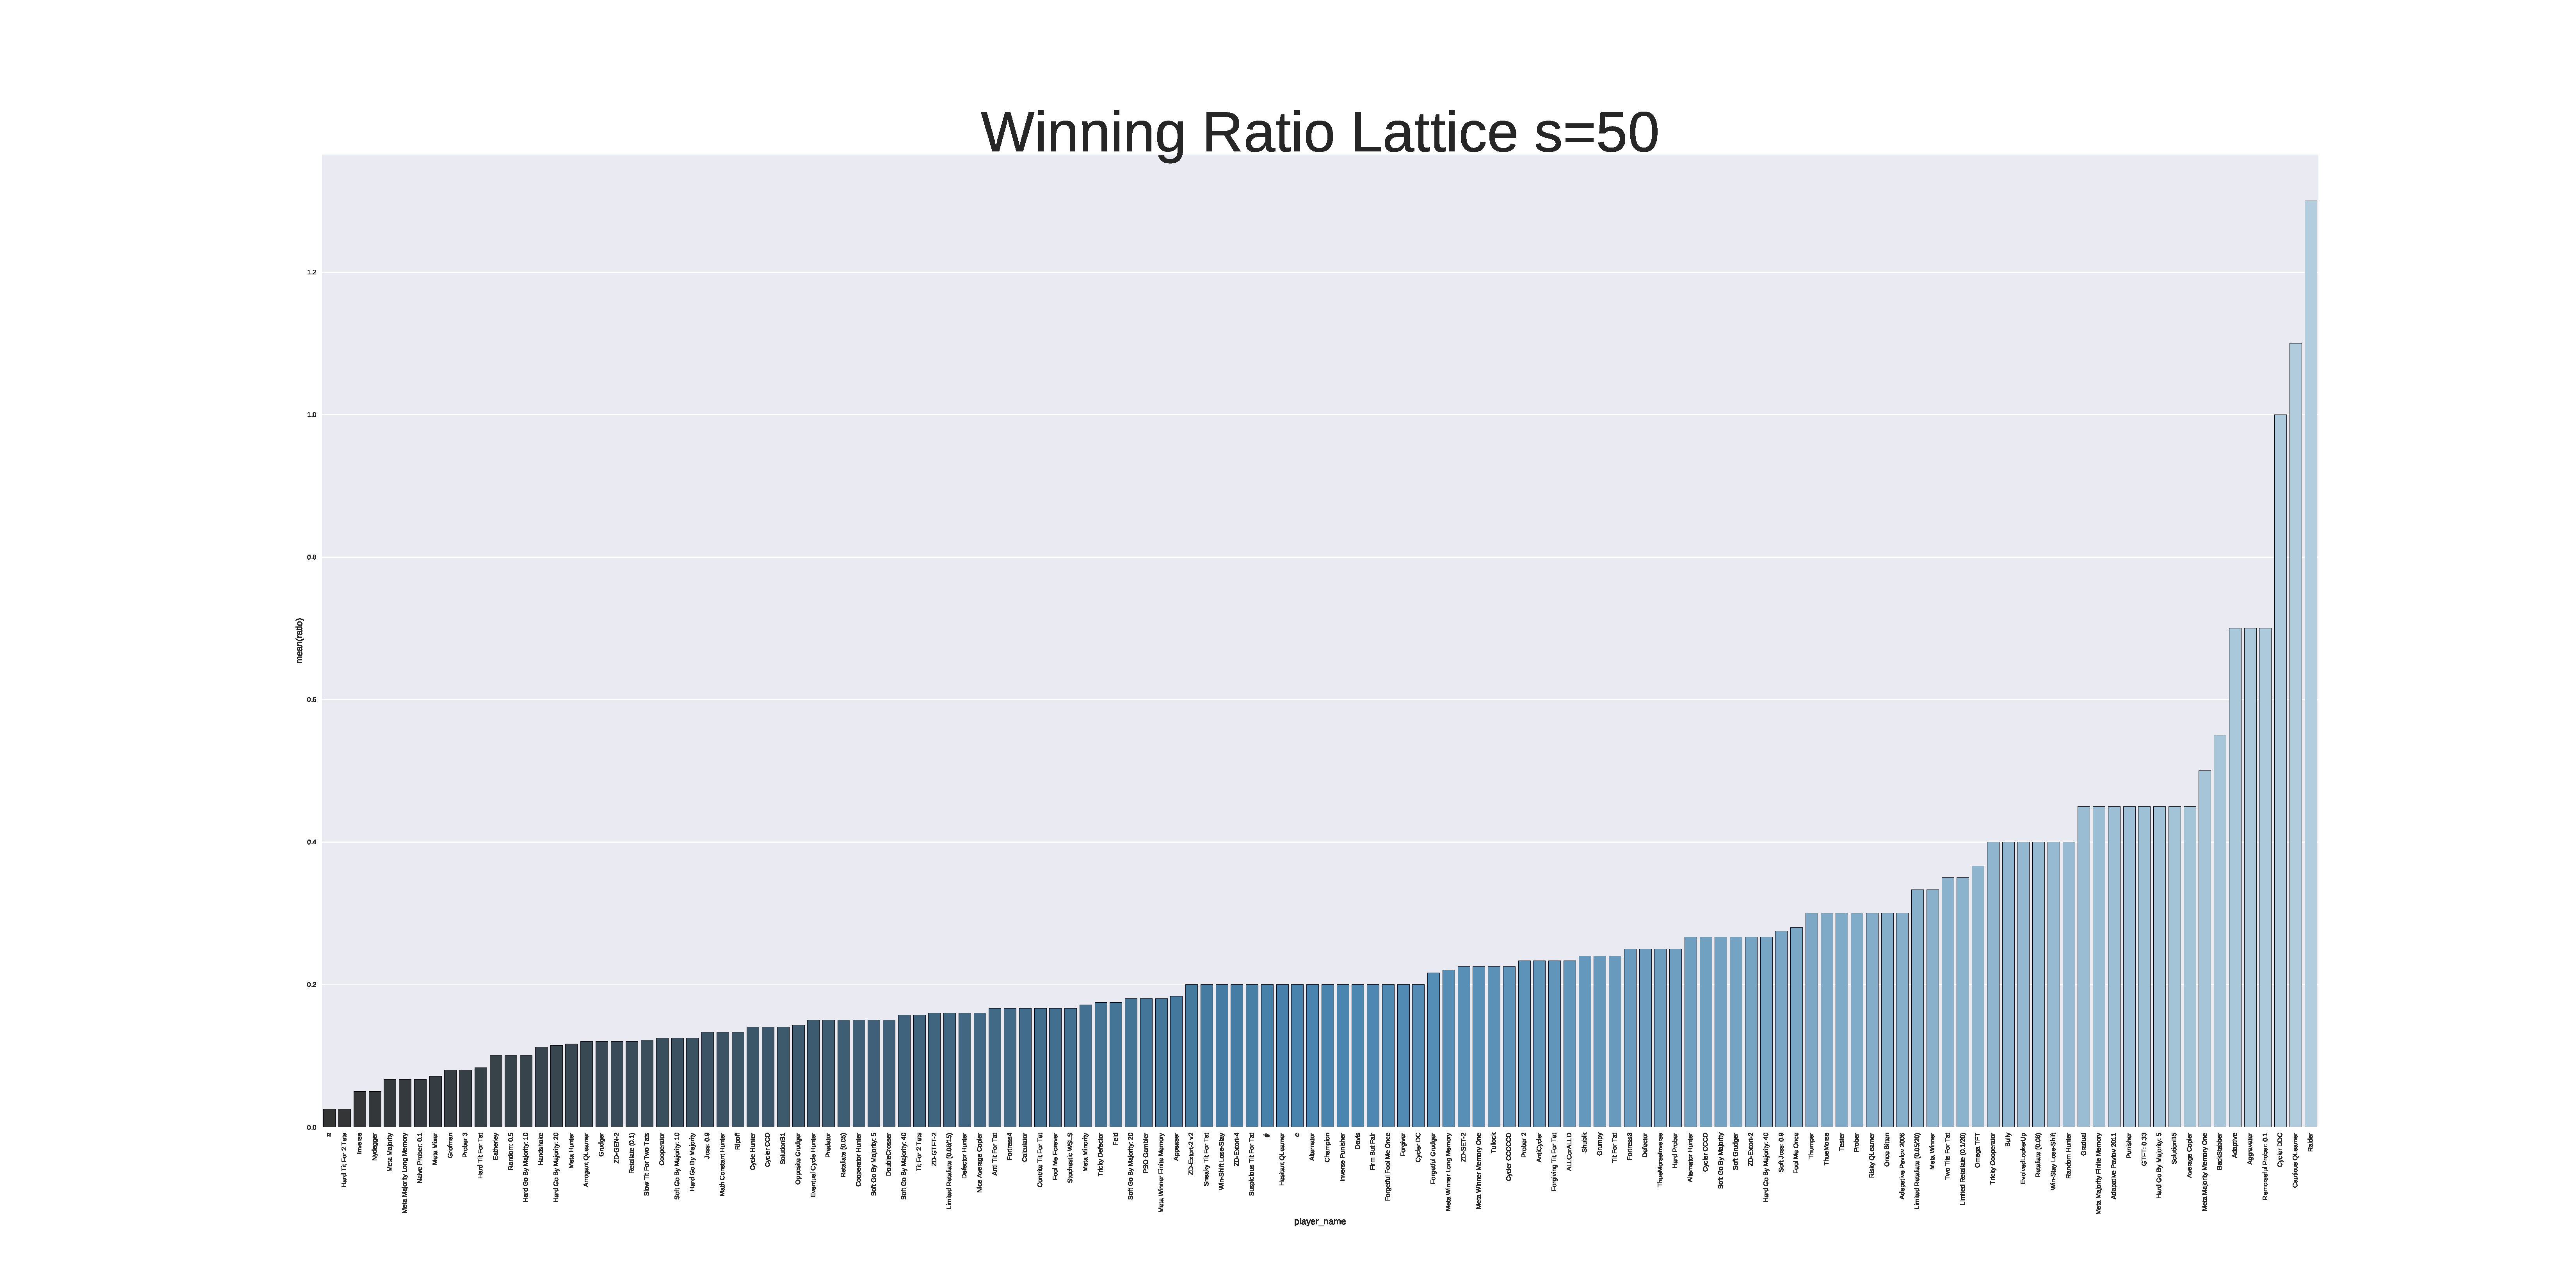
\includegraphics[width=\linewidth]{winners-lattice_fifty.pdf}
    \caption{Winning ration lattice s=50.}
    \end{subfigure}
\hfill
    \begin{subfigure}[t]{1\textwidth}\centering
    \centering
        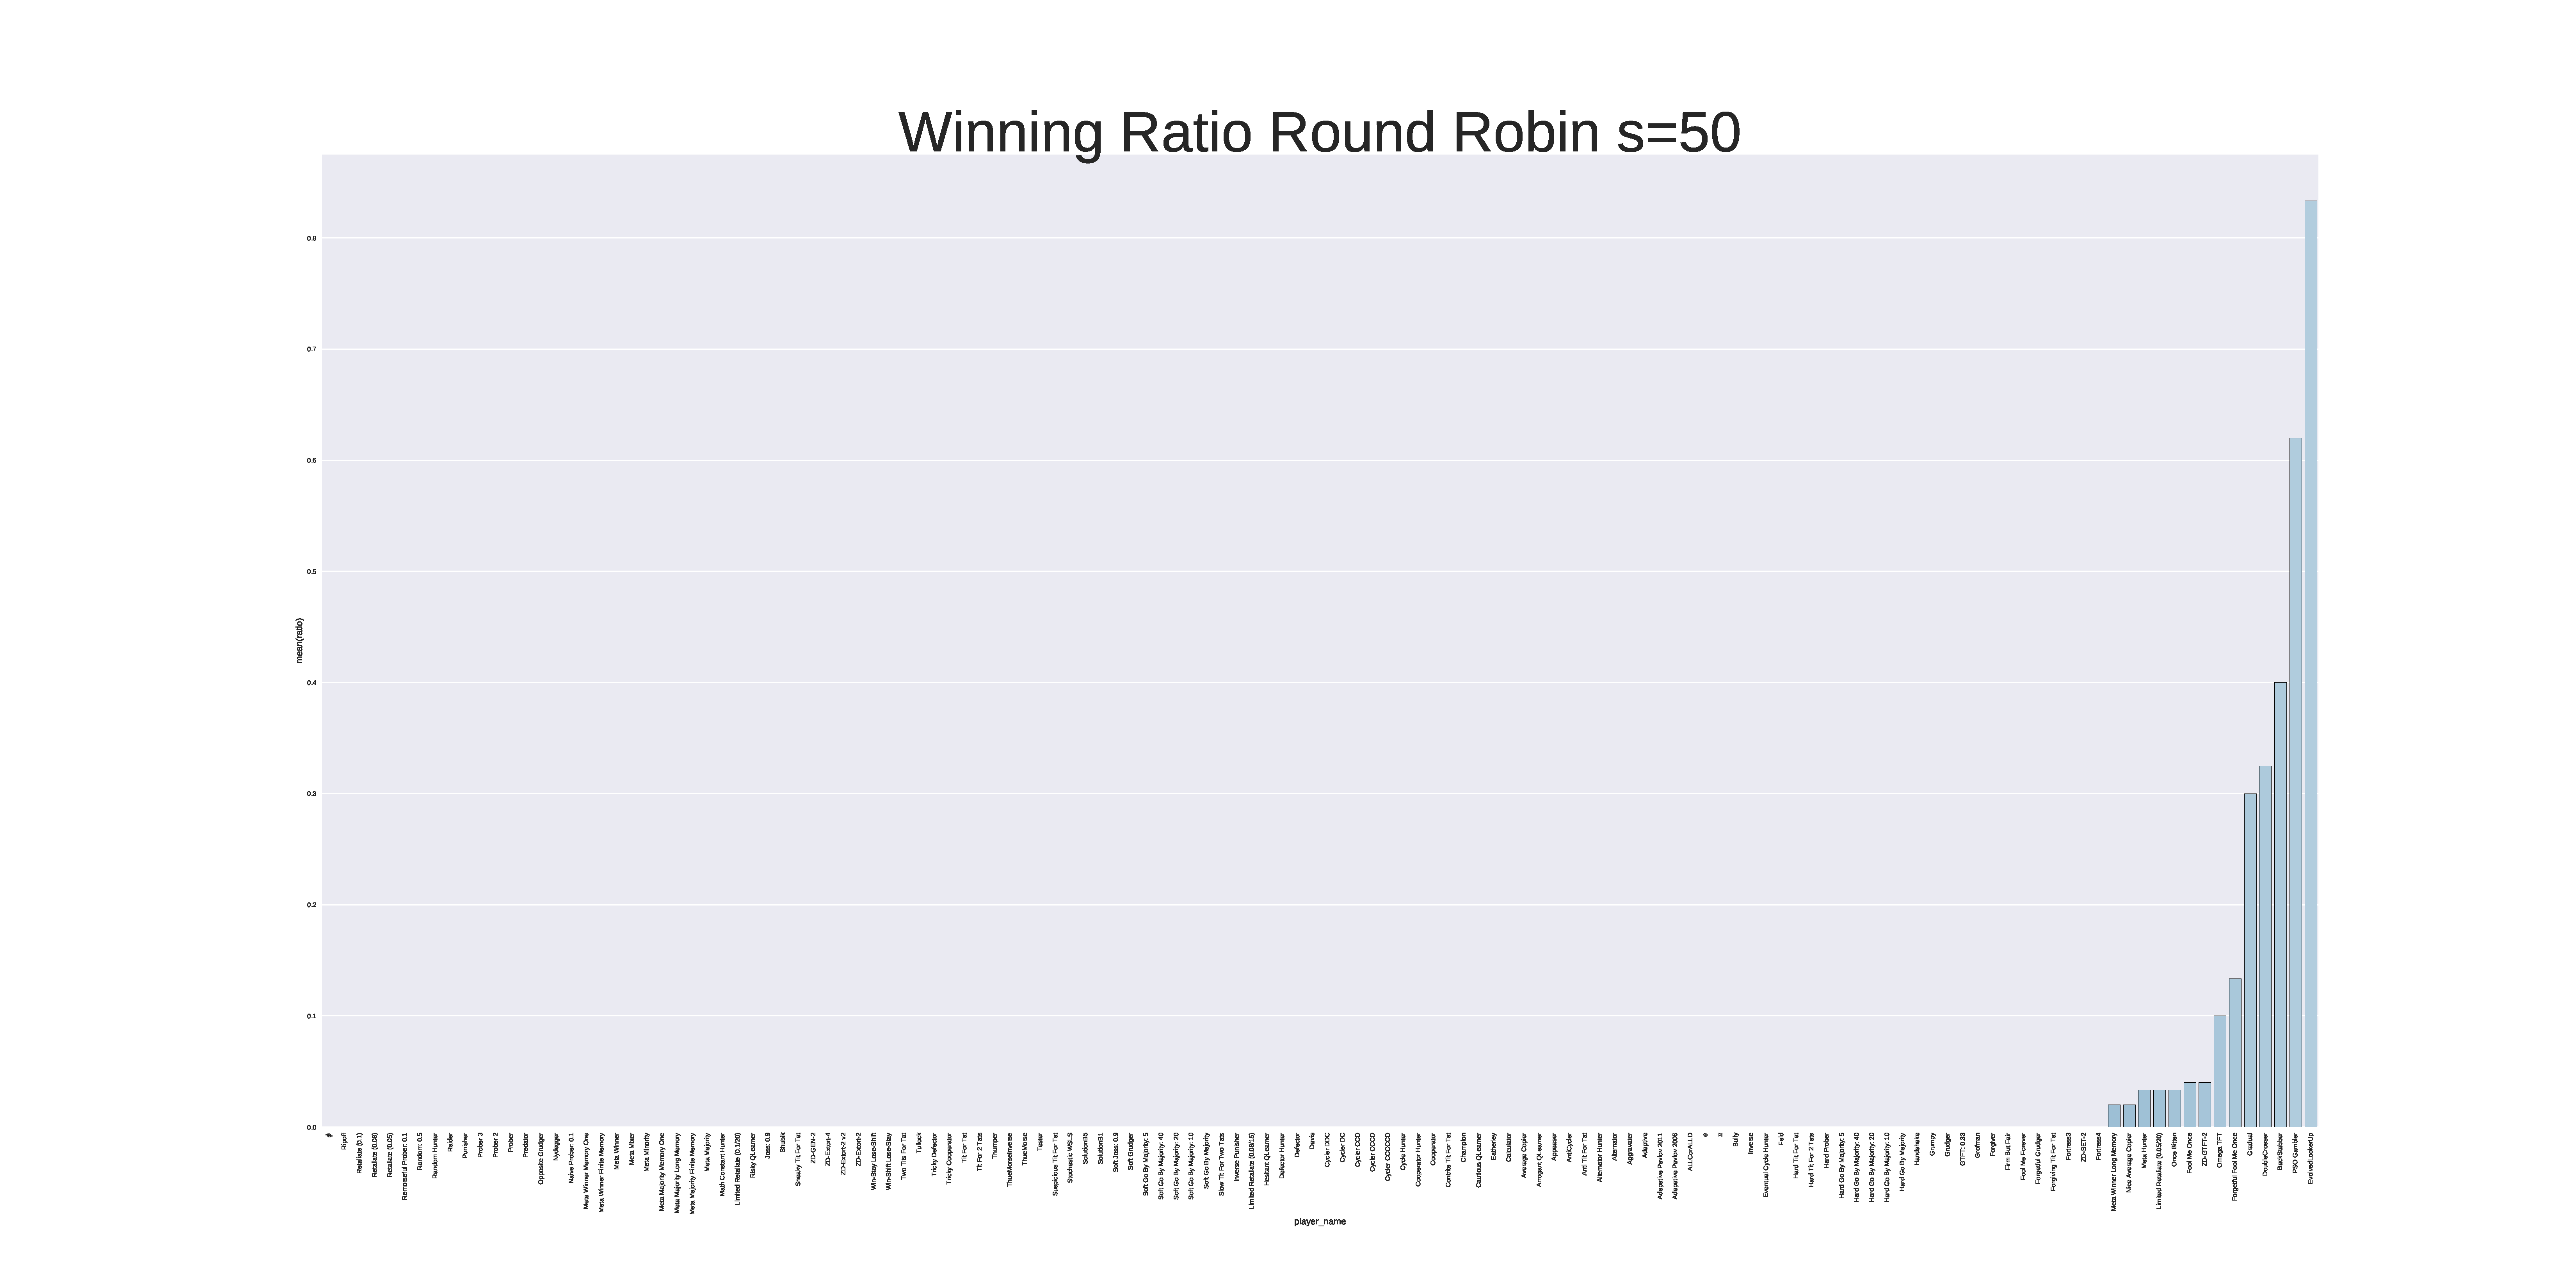
\includegraphics[width=\linewidth]{winners-rr_fifty.pdf}
    \caption{Winning ration round robin s=50.}
    \end{subfigure}
\caption{Winning ratio for all three topologies s=50.}
\label{fig:winning-fifty}
\end{figure}

Now that the winning strategy seem to give us no hind as to how to perform
well in any given random situation we will do further investigation.
The winning ration was plotted against the number of participations of each
strategy and the results are shown in Figure~\ref{fig:winning-ratio-five}
Figure~\ref{fig:winning-ratio-fifty}. A regression line was added to the scatter plots
to be able to visualize and point out any hidden trend.

For \(s=5\) we observe that for the topologies lattice and round robin
the regression line is flat. Indicating that there is no correlation between the
participations and the winning ratio. Thus, for these topologies strategies
that participated for a different number of tournaments could have achieved the
same winning ratio. In the cycle topology, the graph indicates a positive
correlation. For the cycle,
we could guess that the strategies that were ranked first in these topology had high
participating rates as well. This seems to apply for only the specific experiment.

On the contrary, for \(s=50\) cycle and lattice show to have a negative
effect between participations and winning ratio. An unexpected results. Thus, playing
less in these experiments could help you achieve a better outcome. This results
could be fixed because of the neighborhoods. For a round robin topology
participation does not seem to have any effect.

\begin{figure}[H]
\centering

    \begin{subfigure}[t]{1\textwidth}
    \centering
        \includegraphics[width=\linewidth]{wining-ratio-cycle_five.pdf}
    \caption{Winning ration against number of participations cycle s=5.}
    \end{subfigure}
\hfill
    \begin{subfigure}[t]{1\textwidth}\centering
    \centering
        \includegraphics[width=\linewidth]{wining-ratio-lattice_five.pdf}
    \caption{Winning ration against number of participations lattice s=5.}
    \end{subfigure}
\hfill
    \begin{subfigure}[t]{1\textwidth}\centering
    \centering
        \includegraphics[width=\linewidth]{wining-ratio-rr_five.pdf}
    \caption{Winning ration against number of participations round robin s=5.}
    \end{subfigure}
\caption{Winning ratio against number of participating in a tournament
         for all three topologies s=5.}
\label{fig:winning-ratio-five}
\end{figure}

\begin{figure}[H]
\centering
    \begin{subfigure}[t]{1\textwidth}
    \centering
        \includegraphics[width=\linewidth]{wining-ratio-cycle_fifty.pdf}
    \caption{Winning ration against number of participations cycle s=50.}
    \end{subfigure}
\hfill
    \begin{subfigure}[t]{1\textwidth}\centering
    \centering
        \includegraphics[width=\linewidth]{wining-ratio-lattice_fifty.pdf}
    \caption{Winning ration against number of participations lattice s=50.}
    \end{subfigure}
\hfill
    \begin{subfigure}[t]{1\textwidth}\centering
    \centering
        \includegraphics[width=\linewidth]{wining-ratio-rr_fifty.pdf}
    \caption{Winning ration against number of participations round robin s=50.}
    \end{subfigure}
\caption{Winning ratio against number of participating in a tournament
             for all three topologies s=50.}
\label{fig:winning-ratio-fifty}
\end{figure}

\subsection{Average Scores}

The normalized average score is calculated by diving the average score
of each strategy with their participating rates. Then the average score
is plotted against the strategies. As shown in both Figure~\ref{fig:average-score-five}
and Figure~\ref{fig:average-score-fifty}.

For all six experiments the normalized average score seems to has a lot
of variation. Which indicates each strategy performed differently at given
points of the same experiment. These could be because of the opponent or the
whole neighborhood.

Not many conclusions can be made out of this. The high variation could indicate
that our results are complete random.  Unfortunately, this could mean that for
any random situation there does not seem to be a strategy that could
perform equally good.

%Change box plots to violin plots
\begin{figure}[H]
\centering
    \begin{subfigure}[t]{1\textwidth}
    \centering
        \includegraphics[width=\linewidth]{box-plot-cycle_five.pdf}
    \caption{Normalized average score cycle s=5.}
    \end{subfigure}
\hfill
    \begin{subfigure}[t]{1\textwidth}\centering
    \centering
        \includegraphics[width=\linewidth]{box-plot-lattice_five.pdf}
    \caption{Normalized average score cycle s=5.}
    \end{subfigure}
\hfill
    \begin{subfigure}[t]{1\textwidth}\centering
    \centering
        \includegraphics[width=\linewidth]{box-plot-rr_five.pdf}
    \caption{Normalized average score cycle s=5.}
    \end{subfigure}
\caption{Normalized average score for the three topologies s=5.}
\label{fig:average-score-five}
\end{figure}

\begin{figure}[H]
\centering
    \begin{subfigure}[t]{1\textwidth}
    \centering
        \includegraphics[width=\linewidth]{box-plot-cycle_fifty.pdf}
    \caption{Normalized average score cycle s=50.}
    \end{subfigure}
\hfill
    \begin{subfigure}[t]{1\textwidth}\centering
    \centering
        \includegraphics[width=\linewidth]{box-plot-lattice_fifty.pdf}
    \caption{Normalized average score cycle s=50.}
    \end{subfigure}
\hfill
    \begin{subfigure}[t]{1\textwidth}\centering
    \centering
        \includegraphics[width=\linewidth]{box-plot-rr_fifty.pdf}
    \caption{Normalized average score cycle s=50.}
    \end{subfigure}
\caption{Normalized average score for the three topologies s=50.}
\label{fig:average-score-fifty}
\end{figure}

% average score against participations can be added

\subsection{Regression}

Finally, a common methodology when investing factors as predictors is building a
regression model. We are building a model wanting to identify any factor that can
explain the winning ratio and  average score of a strategy.The round robin
topology is not included in this subsection analysis. As explained
above, parameters as average neighborhood score was not monitored. We believe
that in a round robin topology factors like do not have significant effects.
Also round robin topology was mainly used for comparison reasons.

The second model using the normalized average score is the following :

\begin{equation}\label{regmodel}
\begin{split}
normalized\textrm{ }average\textrm{ }score = degree + average\textrm{ }neighborhood\textrm{ }score + \\
clustering + number\textrm{ }of\textrm{ }participations
\end{split}
\end{equation}

The model was used to each of the experiments for lattice and cycle topologies.
The results of models are shown below, Table~\ref{regression} :

\begin{table}[!hbtp]
\centering
\begin{adjustbox}{width=1\textwidth}
\small
\begin{tabular}{@{}|l|l|l|l|l|l|l|l|l|l|l|l|l|@{}}
\toprule
Size & Topology & \multicolumn{2}{l|}{Intercept} & \multicolumn{2}{l|}{degree} & \multicolumn{2}{l|}{average neighborhood score} & \multicolumn{2}{l|}{connectivity} & \multicolumn{2}{l|}{participations} & R-square \\ \midrule
     &          & coef            & p            & coef          & p           & coef                      & p                    & coef             & p              & coef                & p             &          \\ \midrule
s=5  & Cycle    & 0.028           & 0.00         & 0.0559        & 0.00        & -3.763e-06                & 0.043                & 0.0              & NA             & -0.0016             & 0.00          & 0.457    \\ \midrule
     & Lattice  & 0.0064          & 0.00         & 0.0256        & 0.00        & 1.079e-05                 & 0.00                 & 0.0064           & 0.00           & -0.0016             & 0.00          & 0.549    \\ \midrule
s=50 & Cycle    & 0.0025          & 0.00         & 0.0051        & 0.00        & -2.168e-07                & 0.00                 & 0                & NA             & -1.602e-05          & 0.00          & 0.120    \\ \midrule
     & Lattice  & 0.0006          & 0.00         & 0.0024        & 0.00        & 1.033e-06                 & 0.00                 & 0.0003           & 0.00           & -1.601e-05          & 0.00          & 0.216    \\ \bottomrule
\end{tabular}
\end{adjustbox}
\caption{Regression results for model ~\ref{regmodel}}
\label{regression}
\end{table}

In the output we can see that Degree, average neighborhood score and participations
are significant predictors for all the experiments with a \(p\) value less than an 0.00.
Lower than the common alpha level of 0.05
For the cycle topology, average neighborhood score and participations have a negative
coefficients. For example a decrease in participations by one would increase
the average score by 0.0016. Degree on the other hand has a positive coefficient
and connectivity has no effect at all. Furthermore the model for \(s=5\) has
a R-square value of 0.457, thus it only explains 0.4 variation of the data which is
quite insignificant. For \(s=50\) it is even lower at only 0.12.

Finally, for the lattice topology only participations have a negative coefficients.
Thus the only factor with a reverse influence on average score in the lattice topology.
Connectivity is an significant predictor as well with a coefficient 0.0064 and
0.0003 respectively. Though the R-square value is still significant small,
with a value 0.547 and 0.216 respectively.
Even if there are predictors with a significant \(p\) value, the overall
performance of the model is moderate.

%couldnt get winning ration in data frame

\section{Summary}

In this section we will make a summary of all the previous analysis that was made
in~\ref{sub:effects} and list further research we could conduct moving forwards.

From the analysis that was performed in~\ref{sub:winning-ratio}, the wining ratio
for each strategy for all 6 experiments indicated the following :
\begin{itemize}
  \item For the cycle topology of \(s=5\) ZD-GEN-2 had the highest winning ratio
        and for the lattice BackStabber and Meta Majority Memory one
  \item For round robin s=50, most of the strategies finished the experiment
        with winning ratio of zero.
  \item Raider seem to have successful performance in both lattice and cycle \(s=50\)
        and in round robin \(s=5\).
\end{itemize}

An attempt to find any significant reason as to why these strategies outperform
the rest returned the findings below:
\begin{itemize}
  \item Participating rate has a negative effect on the winning ratio for \(s=50\)
        in lattice and cycle topology and a positive in cycle for \(s=5\)
  \item There is high variation is the average score of each strategy for all
        experiments
  \item Regression model for the normalized average score did not return any
        significant results.
\end{itemize}

Even so, Raider stand out we could not produce any valid facts as to why this
was not random and the Raider base on a number of reasons performed so well.
Numerous actions could solve this. Actions that will be taking into consideration
in the experiments to follow. Firstly, the network topologies used have been
simple examples of graph, thus more sophisticated graphs will be used
with different range of neighborhood sizes. Additionally, having a measure of
comparing strategies will be useful. Thus, we will keep track of the cooperating
rate of the strategies in the future.
